\documentclass[../thesis.tex]{subfiles}
  \begin{document}
\chapter{Introduction}\label{cap:introduction}
Improving the way an operator can interact with a robot is a hard challenge in the field of \acrfull{HRI}. The main idea of the project is to solve this problem by using Computer Vision and \acrfull{ML} techniques to recognize some hand gestures made by the operator. In this way, the operator can use the expressive power of his/her hands and their immediacy to communicate with the robot. Moreover, making this idea an interface through the \acrfull{ROS} framework will allow us not to care which robot anyone want to control in the future because it will be enough that it accepts specific messages to work. An example of the idea we want to implement is the one in~\ref{fig:systemArchitecture}.

\begin{figure}[H]
  \centering
  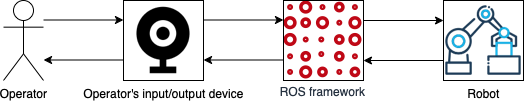
\includegraphics[width=0.7\columnwidth]{systemArchitecture.png}
  \caption{Example of system archicture.}
  \label{fig:systemArchitecture}
\end{figure}

\section{Motivation and objectives}\label{s:motivation-and-objectives}
In recent years the computational power of processors and the ability to deploy \acrshort{ML} models on cheaper and smaller devices has paved the way to interact with computers and robots in a way unfeasible before.\\

The objectives of this internship were to study and develop a solution that would use Computer Vision and Machine Learning techniques to recognize in real-time a set of hand gestures and communicate to a robot which action to execute based on the gesture. I focused on the warehouse's tasks because since 2011 Amazon started using robots inside its warehouses, and nowadays, the number of warehouses that use robots to carry products is fastly growing~\cite{article:bogue2016}. The communication must be via \acrshort{ROS} to make it indifferent from the command receiver. Moreover, a way to describe some \glspl{macro} is implemented to improve the usability experience. To perform all these tasks I delved into the literature looking for what is the state of the art of the \acrshort{HRI}, what are its evaluation methods, and what is the best way to perform a hand gestures recognition task.

\section{Organization}\label{s:organization}
\begin{description}
    \item[{\hyperref[cap:background]{Chapter two}}] describes the background I obtained studying the literature about \acrlong{HRI} and hand gestures recognition.
    \item[{\hyperref[cap:technologies-and-tools]{Chapter three}}] describes the technologies and tools used to implment the solution proposed.
\end{description}

\end{document}
